\chapter{Conclusion}
\label{chapter:conclusion}

%\minitoc
\chapterwithfigures{\nameref*{chapter:conclusion}}
%\chapterwithtables{\nameref*{chapter:introduction}}

\ifthenelse{\boolean{skipConclusion}}{\endinput}{}

This thesis primarely focused on the novel view synthesis issue, mostly with the highly constrained single-view scenario. We skim through in this section over our core contributions, before drawing up  the current 2024 landscape in \ac{AI} and 3D. The last section of this manuscript will be devoted to the perspectives and further work this PhD thesis might lead to. 

\section{Contributions}

This manuscript has adressed in a large extend the single-image \ac{NVS} issue. We built in our first two contributions around latest deep learning architectures to synthesize a novel viewpoint of a static scene from a single source posed image. Our latest project has an industrial primary aim, where novel views are rendered from a scene that was explicitly reconstructed in 3D as a gaussian point cloud.

We started this manuscript by presenting in Chapter \ref{chapter:epipolarnvs} our epipolarNVS architecture. Our main motivation through this work was to propose an innovative way to encode camera pose information in an image-to-image \ac{CNN} for \ac{NVS}. Whereas most of prior work often discretized \citep{kim2020novel} or encoded camera pose information into a low dimensional signal \citep{sun2018multiview}, we rather exploited the epipolar constraint to encode such prior signal. Through a vanilla grid sampling strategy on the source view, we project epipolar lines on a blank RGB image, that was been fed alongside the source image to pose-condition the network. 

We then investigated in Chapter \ref{chapter:epinerf} how epipolar constraints could be bring into a generalizable \ac{NeRF} architecture for single-image \ac{NVS}. Based on \textit{source-aligned} dense feature volume produced from a CNN-encoder, we trained a novel \ac{NeRF}-architecture, termed NeRFeature \ref{subsec:epinerf/method/nerfeature} to produce \textit{target-aligned} features. These \textit{source} and \textit{target-aligned} feature are finally used through an epipolar constraint in a light attention mechanism. We extensively shown in the devoted Experiments section \ref{subsec:epinerf/experiments} how our three-stage training architecture might help generalizable \ac{NeRF}s to better perfrom on single-image \ac{NVS} task.  

Finally, Chapter \ref{chapter:gausssplat} has been entirely devoted to the \ac{NVS} solution we started investigated with CarCutter by Meero few months ago. The camera spin stabilization algorithm allows to render from a 3D \ac{GS} reconstructed scene novel viewpoints which were initially uncomplete and cropped (subsection \ref{subsec:gs-vanilla_gs}). We presented a bunch of improvements to go beyond this first reconstruction in Experiments \ref{sec:gs-experiment}. However, 3D \ac{GS}-based scenes remain prone to floaters artifact when they are rendered at non-training locations. We will push in that direction in a close future to develop a floater removal algorithm. While results are still unperfect for an industrial application, research and open-source projects around \ac{GS} \citep{kerbl20233d} are tremendously prolific and move at a very steady pace for 10 months now \citep{luiten2023dynamic,yang2024gaussianobject,wewer24latentsplat}. 

On top of these contributions, we also introduce in Appendix \ref{chapter:appendix} our very first work, called AdaptativeSR \citep{landreau2022adaptativesr}. There is no direct relationship with the \ac{NVS} but rather with topological considerations in low-resolution 3D meshe structure. Idea was to leverage on the very first differentiable rasterizers that emerged in 2020 \citep{liu2019soft} (before this PhD started) to prune faces of a genus-0 object mesh. By solely relying on 2D binary rendered silhouette mask of such a 3D object, we proposed an effective yet imperfect algorithm to adapt mesh topology. 

\section{IA challenges in 2024}

This section embrasses the most recent issues and trends 3D related \ac{AI} landscape is currently living. This section is not technical but aims to span across the main challenges the scientific community - from academic researchers to tech companies -, but also individuals, will have to face in the months and years to come. 

\subsection{Open-source}
\ac{AI} has been somehow bring into world hands with the release by OpenIA in December 2022 of ChatGPT, an \ac{LLM} based conversational chabot (even throu)

However, underlying technology of \ac{LLM} was already well understood by scientific community years before its release. OpenIA was used to publish (both code and technical notes) on a regular basis their latest advances on their \textit{GPT} models. GPT-2 model (a prior version of ChatGPT) was thus notably permissive from a licence perspective in 2018. Such an openness period has since ended at OpenAI, that now only releases source code on few of its product, as \textit{Whisper}, a general-purpose speech recognition model. \ac{AI} world has witnessed a fundamental chisme in the way research and code should be shared or kept secret. It puts back to back firms that advocate for an open-source access of any significant improvement toward \ac{AI} against those that rather claim for a necessity to keep a proprietary control over technologies and \ac{AI}-based algorithms that could be dangerously misused. MistralAI, HuggingFace or StabilityAI somehow now stand against companies, as OpenIA, Anthropic or MidJourney, that market and distribute \ac{AI} products whose technological foundations are inaccessible to the academic research nor individuals. 

I firmly believe that \ac{AI} research is now supported by an expert and brilliant growing community that is highly motivated by the forthcoming technological and intellectual challenges \ac{AI} is raising. Closed-proprietary \ac{AI} companies will ineluctably be overtaken by  its open source community counterpart. The Figure \ref{fig:conclusion-openclose} highlights such a claim, at least regarding the \ac{LLM} sector. 
\begin{figure}[htb!]
    \center
  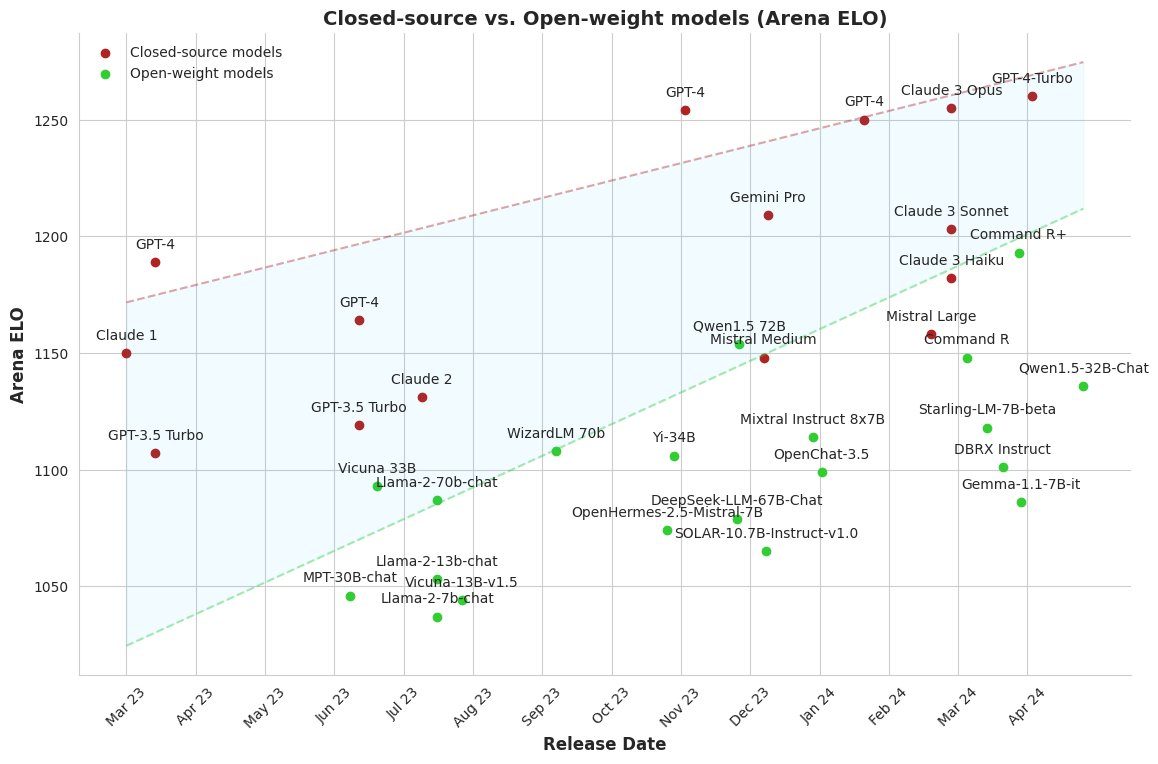
\includegraphics[width=\linewidth]{images/conclusion/open-close.jpeg}
  \caption{\textbf{LLMs ELO score based on human ratings.} Such graphs is built on a regular monthly basis thanks to \citep{chiang2024chatbot} work. It seems that open models now has a 6 to 10-month lag, againt more than years when GPT-4 was released.}
  \label{fig:conclusion-openclose}
\end{figure}

While 3D \ac{AI} is not as concerned as \ac{LLM} by such a trend, we currently observing an increasing number of startups raising funds to either defend one of the two models. StabilityAI, an already esteemed companie in \ac{AI} landscape for its diffusion models \citep{esser2024scaling}, has for instance recently made public a significant number of single-image 3D reconstruction models \citep{tochilkin2024triposr,voleti2024sv3d}. 

\subsection{Fundation models and environmental issue}

Almost all modalities, from text (\textit{Mistral7B} by MistralIA, \textit{Llama2} by Meta, \textit{Claude3} by Antropic, \textit{GPT-4} by OpenIA) to image (\textit{Stable Diffusion 3} by StabilityAI, \textit{DALL.E 3} by OpenIA, Midjourney \textit{V6}) and video (\textit{SoRA} by OpenIA, \textit{Gen-2} by Runway), have now get their fundation models. The 3D is maybe one of the very last domain, with audio, not to have done so.\footnote{We exclude here latest work in single-image 3D reconstruction since they are still limited to centric object at low resolution.} But domains related to \ac{VR}, video games or animation have not yet witnessed the \ac{AI} revolution text and image have faced since few years. OpenAI CEO Sam Altman has indeed recently tweeted in April 2024 toward such an affirmation: "movies are going to become video games and video games are going to become something unimaginably better". Hard to not see here the growing importance 3D is gonna have in the coming years. 

However, while an increasing numbers of models are now freely available, \ac{GPU}s ressources required to train or even perform inference such models (that gets hundreds of millions to tens of billions learnable parameters) remain immensely substantial. One of the latest MistralAI model, called \textit{8x7B}, thus requires almost 700GB of vRAM \ac{GPU} for training (an 8-A100 \ac{GPU}s cluster would not be sufficient here) as shown on Table \ref{tab:gs-mistral_requirement}. 

\begin{table}[htp!]
  \caption{\textbf{ Mistral 8x7B model} Half and full precision vRAM GPU requirements for training. Figures from \href{https://huggingface.co/docs/accelerate/main/en/usage_guides/model_size_estimator}{HuggingFace Model Memory Calculator}}
  \label{tab:gs-mistral_requirement}
  \centering
  \begin{adjustbox}{width=\linewidth}
  \begin{tabular}[h]{c||cccc}
  \hline 
   - &  \textit{Model} & \textit{Gradient calculation} & \textit{Backward pass} & \textit{Optimizer step} \\
  \hline 
  \textbf{float16} \textit{(half)} & 174.4GB  & 261.7GB & 348.9GB & 348.9GB\\
  \textbf{float32} \textit{(full)} &  174.4GB  & 174.4GB & 348.9GB & 697.9GB \\
  \hline 
  \end{tabular}
  \end{adjustbox}
\end{table}
Factorial Funds estimates in one of its \href{https://www.factorialfunds.com/blog/under-the-hood-how-openai-s-sora-model-works}{report} that between $4.2K$ and $10K$ Nvidia H100 \ac{GPU}s has been required for a whole month to train the latest text-to-video OpenAI \textit{SoRa} models. With a 700W power per \ac{GPU}, \textit{SoRA} training has consummed over a month as much as electricity as a french individual in 12 years. The same note also reports that a single H100 is able to produce a 5 minutes video within an hour. If such an innovative technology is proned to be publicly avalable in months and years to come, Fcatorial Funds estimates that OpenIA will require approximately 720,000 H100 GPUs to meet global demand.\footnote{Based on 50\% \ac{AI}-generated videos on TikTok for a daily basis and 15\% on Youtube.}

Finally, actual trend from NVDIA regarding its \ac{GPU} development is not pushed toward frugal energetic consumption. Main goal is rather to always push for better FLOAPS performance: while next \ac{GPU} Blackwell generation from NVIDIA, called B100 and B200, are going to be 25 times faster than H100, they will also be set at a 1000W power requirement. 


\subsection{AI Ethics} 

Over the past five years, \ac{AI} has made significant progress at a blistering pace. As \ac{AI} capabalities become stronger every day, so does the need to tackle its associated ethical delemmas. 

Ethics is somehow one of the main argument set ahead by companies advocating for the exclusive ownership of their \ac{AI} algorithms and products. Ensure that such source codes would be kept away from hands of those who would use it improperly for malicious reasons. Whereas \ac{AI}-based algorithms in audio or images were not sufficiently good few years ago to deceive the human eye or ear, deck has been thoroughly reshuffled lately. Fortunately \ac{AI} is not restricted in its application to generative content creation. Decision-making powers granted by \ac{AI} are gradually being adopted more widely, as in the medical field for the detection of cancerous tumors (Owkin), or in more controversial areas such as for military applications (Anduril).

OpenIA presented in March 2024 one of its latest product, called \href{https://openai.com/blog/navigating-the-challenges-and-opportunities-of-synthetic-voices}{Voice Engine}. A 15 seconds audio recording is now sufficient to extremely accurately clone a human voice through this \ac{AI}. If OpenAI insists on positive paths and possiblities offered by such a technology (for live translation, to help disabled people with oral disorders), the firm also conceeds that its product brings massive scams threats such telephone frauds or identity thefts. 

First produced deepfakes appeared in 2017 were originally refering to videos where face on a video have been artificially altered by AI to assume the appearance of someone else. The definition has since broadened significantly. Microsoft even release on April 2024 a technology called VASA-1 \citep{xu2024vasa1}, that enables voiced deepfake generation from a single image. As OpenAI a month before, Microsoft already communicates on potential threats and misusages VASA-1 could be involved in. No public release has been announced yet. 

Google developed mid-2023 SynthID, a tool that enables to watermark \ac{AI} generated images and audios. It thus imlicilty allows to protect original human content creation. Decision-making political authorities and parliaments across the world now start and urges their partners to regulate and give \ac{AI} a coherent legal framework. The AI Act has been ratified in Europe in February 2024 and set to take effect in 2025. It will impose a certain level of transparency regarding training data that were used to train any foundation models, or some biais studies regarding results such \ac{AI} models can deliver. The US government does not have such a similiar AI Act yet. 


\section{Perspectives and further work}
We present in this very last section few perspectives as well as further research work that might be investigated following this PhD thesis. We tried, as much as we could, to draw parallels and connections between current 3D \ac{AI} research and industries. 

\subsection{Further work}
This thesis extensively tried to integrate (and leverage on) geometric priors and constraints into deep neural architectures. Only few works intended to do so when we started delving into epipolar considerations years ago. \ac{NVS} has been first tackled through an image-to-image \ac{CNN} in this thesis, leaving the physical image formation process and its inherant 3D-2D projection apart. Our second contribution gets closer from the 3D world, by building a feature epipolar based attention mechanism in a generalizable \ac{NeRF} architecture. However, it exists substantial rooms for further improvements. 

% Single image 3D reconstruction.
3D \ac{AI} research is currently extremely prolific when it comes to deal with the single-image 3D reconstruction (and thus inherently \ac{NVS}). Within the last 6 months, at least three extremely powerful and serious project has been released:  One-2-3-45++ \citep{liu2023one2345++} in November 2023 ,TripoSR \citep{tochilkin2024triposr} in March 2024, InstantMesh \citep{xu2024instantmesh} in April 2024. Fomers were outperformed by the latest InstantMesh. While \ac{NVS} would not anymore be addressed as it was in future, digging into the single-image 3D reconstruction is fore sure a challenging yet intringuing research path to explore. To the best of our knowledge, none of them tries to either integrate symmetry prior nor epipolar constraints in their architecture.


% mixing diffusion and 3D for single-image NVS
While we extensively relied on \ac{NeRF} in our EpiNeRF contribution, latest advances in diffusion-based models enable to adress single image \ac{NVS} under the same assumptions as ours (unique source viewpoint, rich and diverse dataset as ShapeNet \citep{chang2015shapenet}). In this way, NeRFDiff \citep{gu2023nerfdiff}, Diffrf \citep{muller2023diffrf} or GeNVS \citep{chan2023genvs} mixed both 3D radiance fields consideration with large diffusion models to adress our issue. 

However, architectures remain complex to train and rendering time requirements prevents from real time inference. These work are also mostly developed by private compagnies that do not release their course code. In this way, NeRFDiff has been partially developed by Apple and GeNVS by Nvidia, but neither one's code is publicly available. Current research therefore somehow suffers from the lack of open-source single-image \ac{NVS} code\footnote{We discard from our point latest single-image 3D reconstruction as they cannot deal with complex and large datasets that are not object centric such as CO3D \citep{reizenstein2021common}or RealEstate10K \citep{zhou2018stereo}.}. It would thus be worthwhile pursuing research on how diffusion-based models and \ac{NeRF}/\ac{GS}-based \textit{3D explicitness} could coexist and benefit one from each other in a unique \ac{NVS} architecture.

If \ac{NeRF} suffers from these millions of queries needed to render an image, current interest in \ac{GS}-based technology alongside the swift advances on diffusion models should allow to design an effective yet fast single-image \ac{NVS} architecture. Which lead to our last further research direction. 

% Generalizable GS - for a single image / in high quality. 
Finally, one could try to delve into a generalizable \ac{GS}-based framework for high-resolution single-image \ac{NVS}. While generalizable \ac{NeRF} architectures exist since few years now \citep{yu2021pixelnerf,li2022symmnerf,lin2023vision} for such an issue, images resolution ($64\times 64$, up to a$512\times 512$) and rendering speed are still too low. Research around \ac{GS} seems to currently follow a quite similar path to the \ac{NeRF} when they appeared. \ac{GS} weaknesss from the seminal paper \citep{kerbl20233d} are thus subject to plethoera of works over the last few months (as \ac{NeRF} lived since 2021/2022): regarding COLMAP dependencies for camera poses \citep{fu2023colmapfree}, on number of images \citep{xiong2023sparsegs,yang2024gaussianobject}, model weights reduction \citep{niedermayr2023compressed}, training and inference time \citep{fan2024instantsplat}, rendering quality \citep{yu2023mip} , dynamicity \citep{luiten2023dynamic} or graphics attributes \citep{wu2024deferredgs}.  

However, being able to leverage on \ac{GS} quality and rendering performance for highly diverse datasets as we did with NeRF \citep{landreau2024epinerf} with ShapeNet \citep{chang2015shapenet} has barely been tackled, and just in the past few months. Some works as pixelSplat and latentSplat positioned in such a direction, but it still required two images as input to perform the novel viewpoint generation, and iamge resolution is still limited to $256\times 256$. One could therefore design a way to properly image-condition a generalizable gaussian point cloud for the high-resolution single-image \ac{NVS} issue. It would eventually induce to increase the number of learnable attributes for each gaussian primitives, as research on dynamics scene did with 4D gaussians primitives \citep{luiten2023dynamic,gao2024gaussianflow}.  


\subsection{Trends and applications in 3D}
Applications of \ac{AI} to industry has undergone since 2022 a significant revolution regarding content generation from both an image and \ac{LLM} perspective. Recent advances in \ac{LLM} and diffusion-based modèles over the last two years have enable the creation of countless tech startups. 

Wheareas all application domains are impacted by such a rush towards \ac{GenAI} models, the later term primarely refers to text and image \ac{AI} generative models. Applications that involves this extra dimension, either in time with video or space with 3D, are thus relatively underadressed in the industry, even through an increasing number of companies are currently developing products around videos and 3D, as OpenIA with \textit{SoRA} or LumaAI. The 3D domain, in its broadest sense, is set for an unavoidable boom in industry for the coming months and years. We skim through this section over some of the latest trends and application to come in the 3D-\ac{AI} related world. 


\noindent \textbf{Immersive web interaction.} It exists a tremendously number of domains where online 3D web visualization could bring the user experience a step further. The e-commerce industry is one of them. What's about being able to closely and smootly inspect every angle of any pair of shoes on  marketplaces or any car on a dealership website ? Same idea stands for the whole fashion industry, where 3D virtual try-on is gradually taking an increasingly significant share. However, almost all virtual try-on solutions currently leverages 2D diffusion-based models. While third dimension is still often ignored, generated images for virtual try-on often lake of details or structural conherences with challenging poses. Being able to truly account on the inherent 3D structure of any objects to build an industrial product is thus a promissing path several companies such as \href{https://www.graswald.ai/}{Graswald}, \href{https://wanna.fashion/}{WANNA} and \href{https://www.car-cutter.com/}{CarCutter} are currently investigating. 

\noindent \textbf{Biology and medical.} NVIDIA CEO Jensen Huang rencently predicted that digital biology will be "one of biggest revolutions ever". Digital biology encompasses a very wide range of fields, as genomics, proteomics or cell engineering. Biology is at the verge of becoming digitalized, and thus being adressed as an engineering problem, where \ac{AI}, computer science and extremely large databases can met. Time as flied in computational genetics since the 1990s Human Genome Project took 13 years and a 3.8 billion dollar investment to sequence the 92\% of the human genome. Started in 2018 by DeepMind/Google, the AlphaFold project (now at its third iteration) has led to groundbreaking progress in 3D protein's 3D structure and drug discovery. Its associated AlphaFoldDB, a 200 million massive collection of predicted proteins structure, should keep helping academics and industries (as Owkin) to leverage on \ac{AI} to better apprehend virus or cell behaviours in order to find new cancer treatments, vaccines or accelerate clinical trials. However, medical imagings and 3D CT scans would definitely also benefit from latest 3D \ac{AI} advances. World most powerful IRM machine, called Iseult and led by the CEA, has unveilved on April 2024 its very first results. Brain images that are now obtained from this 11.7T IRM now reach a never achieved resolution, as depicted on Figure \ref{fig:conclusion-ceaiseult}.

\begin{figure}[htb!]
  \center
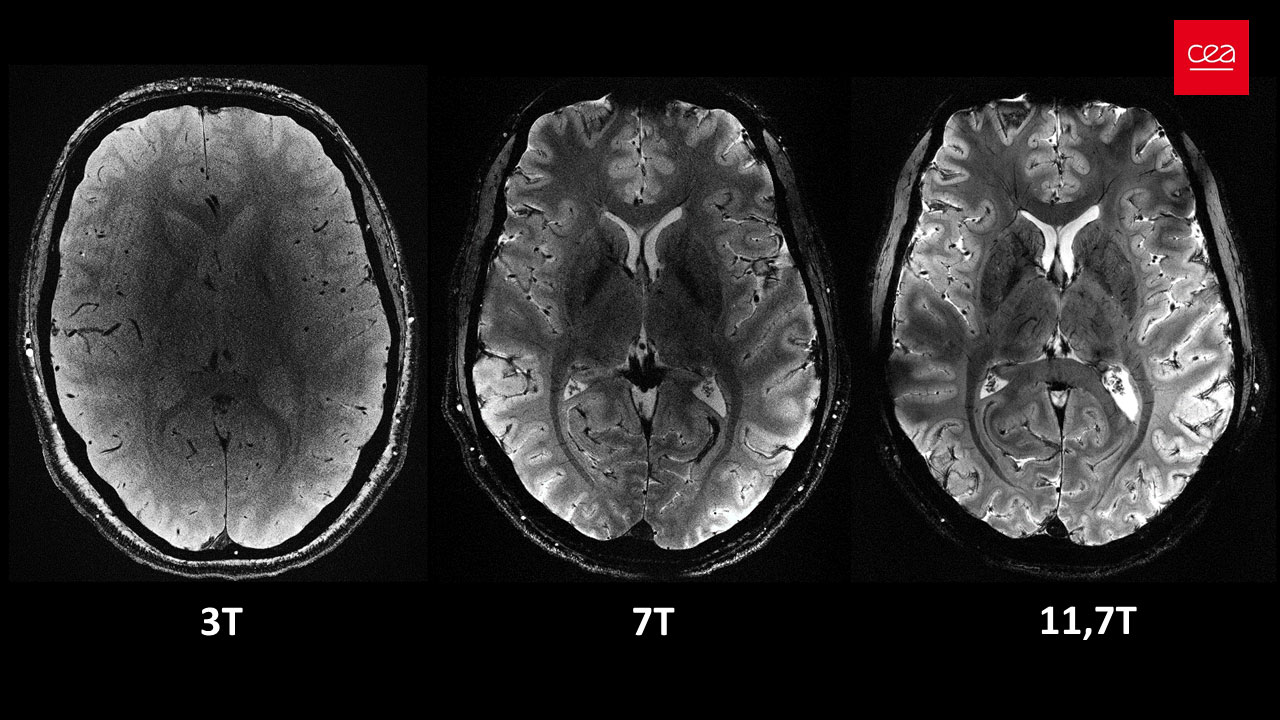
\includegraphics[width=\linewidth]{images/conclusion/cea-iseult.jpg}
\caption{\textbf{Axial sections of the human brain.} Most common IRM machines in hospital has a 3T magnetic field power, leading to brain image on the extrem left. While only a couple of IRM reach 7T in the world, latest CEA Iseult IRM is able, with its unique 11.7T magnetic field, to deliver outstanding results, without no increase in time exposure.}
\label{fig:conclusion-ceaiseult}
\end{figure}

Extremely high resolution images allowed by such an IRM machine,combined with latest \ac{AI} advances should therefore bring medical imaging and 3D organs reconstruction to an unprecedented level in a near future. 

\noindent \textbf{VR/AR and LiDAR.} \ac{VR} and \ac{AR} have a long standing 50 year history. Recent advances in \ac{NeRF} paved the way for some VR oriented work as VR-NeRF \citep{xu2023vr}, that enables real-time dual 2K generation through walkable spaces in virtual reality. Apple's VisionPro mixed-reality headset released in 2023 (commercially marketed as an \textit{spatial computer}) is going to have a massive influence on how \ac{VR} and \ac{AR} are consumed on a daily basis by individuals. Corresponsing OS, termed \textit{visionOS} will enable developers and researchers to build upon such a {spatial computer} for 3D and \ac{CGI}-based applications.

LIDAR sensors are now integrated in almost all flagship smartphones, opening a vast field of research and development over highly-detailed 3D reconstruction. Chinese based startup \href{https://www.xgrids.com/}{XGRID} aims in this way to develop a LiDAR, multi-SLAM and \ac{GS} based solution to build realistic large 3D scenes, in a close future at street or city level. Such ultra-realistic scenes might then be processed through \ac{AI} and conventional graphics and game engines such as Blender, Maya or UnrealEngine. 

\noindent \textbf{Animation and video games.} Finally, animation and video games industries are going to imminently experience a substantial revolution. Processes that holds since decades to animate 3D caracters or render highly-detailed \ac{CGI} scenes are going to be disrupted by \ac{AI}. From storyboarding to 3D modeling and animation, crafting a qualitative cartoon or an animated movie takes months and even years, with dozens of different skilled jobs involved. \ac{AI} and 3D will streamline these costfull production piplines. Latest advances in 3D meshes and \ac{GS}-based rigging and animation \citep{qian2023gaussianavatars,li2024animatablegaussians} confirms that both animation and video would not be produced as they currently are in a near future. 

\ac{CGI}s that are heavely used in the film industry will experienced major advances too thanks to the latest neural rendering fields and graphics research. \ac{GS}-based methods that aims to tackle texture, shading or lightning issue have already been published \citep{jiang2023gaussianshader,wu2024deferredgs} and associated 3D scene can even be manually corrected and modified through \href{https://github.com/aras-p/UnityGaussianSplatting/}{Unity UnrealEngine add-on}. 


